72. \begin{figure}[ht!]
\center{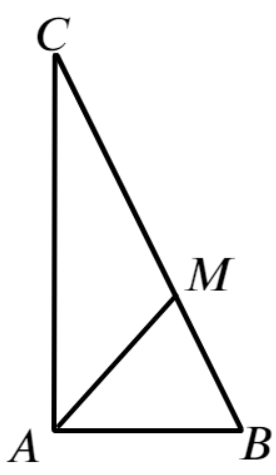
\includegraphics[scale=0.35]{g9-72.png}}
\end{figure}\\
По свойству основания биссектрисы имеем соотношение $\cfrac{AB}{AC}=\cfrac{BM}{MC}=2:4=1:2.$ Пусть $AB=x,\ AC=2x,$ тогда по теореме Пифагора $x^2+4x^2=(2+4)^2,\ x^2=\cfrac{36}{5}.$ Посчитаем площадь треугольника двумя способами: $S=\cfrac{1}{2}AD\cdot6=\cfrac{1}{2}x\cdot2x,$ откуда $6AD=2\cdot\cfrac{36}{5},\ AD=\cfrac{12}{5}.$\\
